%%%%%%%%%%%%%%%%%%%%%%%%%%%%%%%%%%%%%%%%%
% Beamer Presentation
% LaTeX Template
% Version 1.0 (10/11/12)
%
% This template has been downloaded from:
% http://www.LaTeXTemplates.com
%
% License:
% CC BY-NC-SA 3.0 (http://creativecommons.org/licenses/by-nc-sa/3.0/)
%
%%%%%%%%%%%%%%%%%%%%%%%%%%%%%%%%%%%%%%%%%

%----------------------------------------------------------------------------------------
%	PACKAGES AND THEMES
%----------------------------------------------------------------------------------------

\documentclass{beamer}
\usepackage{lmodern,textpos,hyperref,graphicx,booktabs}
\usepackage[ddmmyyyy]{datetime}

\mode<presentation> {
\usetheme{Dresden}
\usecolortheme{beaver}

\definecolor{stanfordBeige5}{RGB}{251,249,249}
\definecolor{stanfordRed}{RGB}{140,21,21}
\definecolor{stanfordBlack}{RGB}{46,45,41}
\definecolor{stanfordRedText}{RGB}{132, 0, 0}
\setbeamercolor{institute in head/foot}{fg=stanfordRedText}
\setbeamercolor*{palette tertiary}{use=structure,fg=white,bg=stanfordRed}
}

\title[Worker--Centric Markets]{Designing Worker--Centric Labor Markets} % The short title appears at the bottom of every slide, the full title is only on the title page

\author{Ali Alkhatib}
\institute[Stanford/FUSE Labs] % Your institution as it will appear on the bottom of every slide, may be shorthand to save space
{
Stanford University, FUSE Labs \\ % Your institution for the title page
\medskip
\texttt{ali.alkhatib@cs.stanford.edu\\@alialkhatib\_} % Your contact info
}

\date{\usdate{\formatdate{13}{11}{2015}}}
% \newdate{date}{13}{11}{2015}

% \date{2015,1,3} % {1}{3} % Date, can be changed to a custom date

\begin{document}

\begin{frame}
\titlepage % Print the title page as the first slide
\end{frame}

\begin{frame}
\frametitle{Roadmap} % Table of contents slide, comment this block out to remove it
\tableofcontents % Throughout your presentation, if you choose to use \section{} and \subsection{} commands, these will automatically be printed on this slide as an overview of your presentation
\end{frame}

%----------------------------------------------------------------------------------------
%	PRESENTATION SLIDES
%----------------------------------------------------------------------------------------

\section{Personal background}
\begin{frame}
  \frametitle{Personal background}
  \begin{itemize}
    % \item Human--Computer Interaction Group
    % \begin{itemize}
    \item Computer Science at Stanford
    % \end{itemize}
    \item FUSE Labs (Microsoft Research)
    \item Collective action (\href{http://www.wearedynamo.org}{Dynamo})
    \item Anthropology at UC Irvine
  \end{itemize}
\end{frame}

\section[Vision]{Vision of cooperatives}
\begin{frame}
\frametitle{[my] Vision of cooperatives}
\begin{itemize}
\item
We all want to see better ``gig'' labor markets.
\item 
Laws protecting these workers have been slow to emerge.
% (Also, some of the work we've done has turned up that workers might not want the entrenched solutions that worked for marginalized workers in the early 20th century)
\item
Ideas can propagate faster than laws and regulations can.
\item
Let's \textbf{demonstrate} that cooperative markets can compete with adversarial ones.
\end{itemize}
% We have outsize influence on the world.
% \begin{itemize}
% \item I can 
% \end{itemize}
\end{frame}

\section[Fieldwork]{Fieldwork}
\begin{frame}
\frametitle{Fieldwork}
\begin{enumerate}
\item
Find participants --- \textit{spending weeks making inroads}
\item
Participant--observation --- \textit{early mornings working dispatch}
\item
Participatory design --- \textit{designing with \textbf{partners}, not clients}
% \item
% Iteration
\end{enumerate}

\end{frame}

\section[Lessons]{What we've learned}

\subsection[]{Intangible}
\begin{frame}
  \frametitle{What we've learned}
  \framesubtitle{Design considerations}
  Important issues for increasingly marginalized workers:
  \begin{itemize}
    \item
    How to design for constructive feedback
    \item
    The social dilemma of work dispatch
    \item
    Managing customer expectations
    % \item
    % Protecting vulnerable workers
    % \item
    % Reconciling worker self--identity
    \item
    More
  \end{itemize}

\end{frame}



\subsection[]{Tangible}
\begin{frame}
  \frametitle{What we've learned}
  \framesubtitle{Things you can run}
  Mock--up of a mobile app designed with workers and advocacy groups as \textit{peers}
  \begin{figure}
    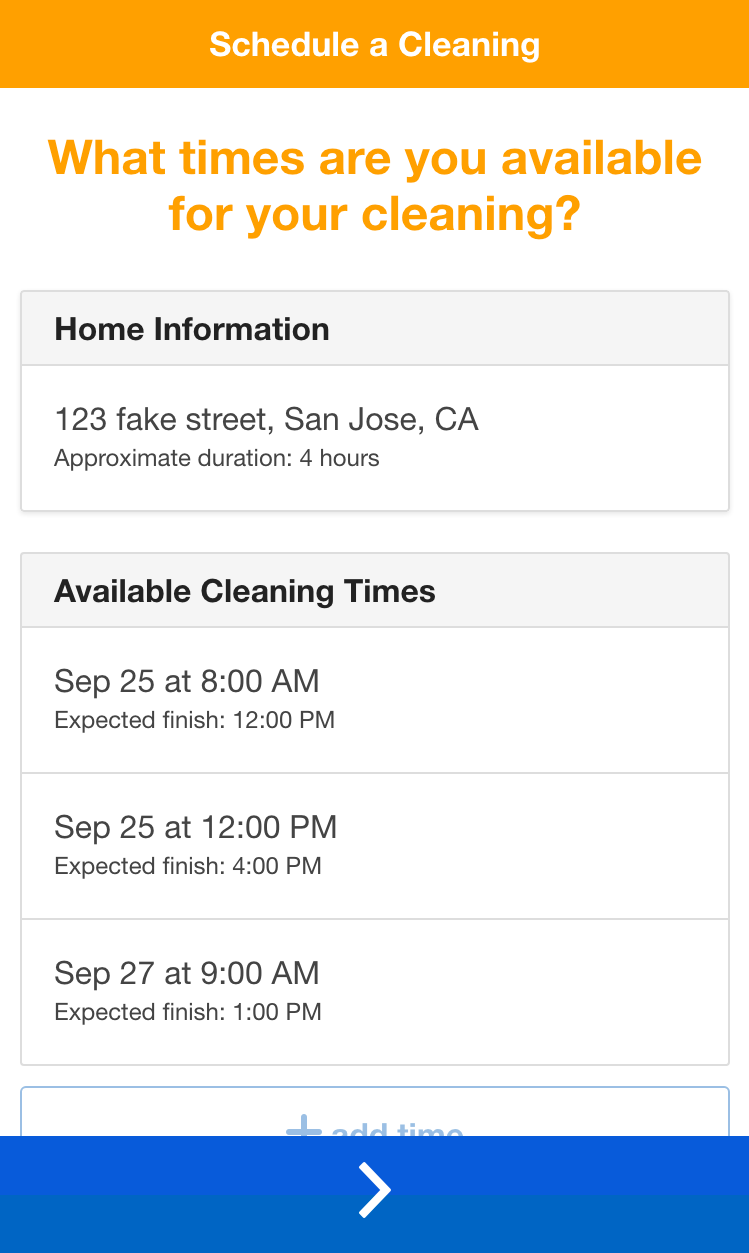
\includegraphics[width=0.25\linewidth]{figures/scheduling}
    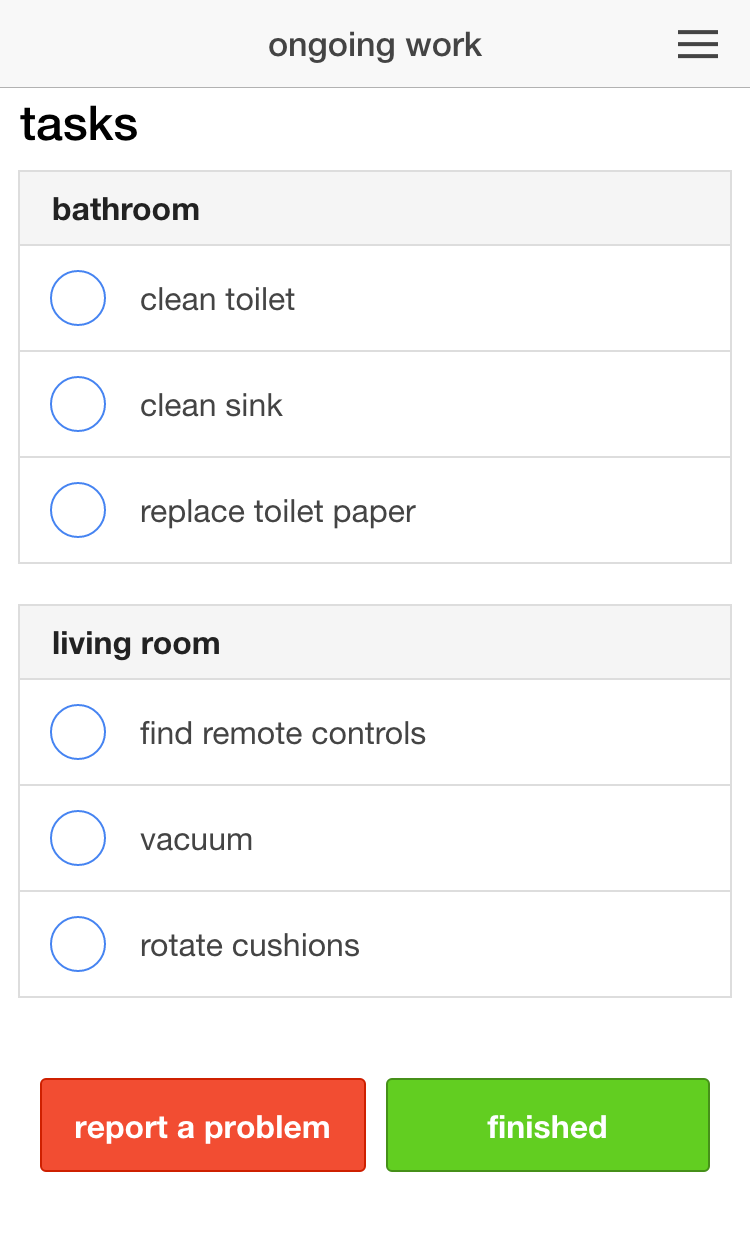
\includegraphics[width=0.25\linewidth]{figures/checklist}
    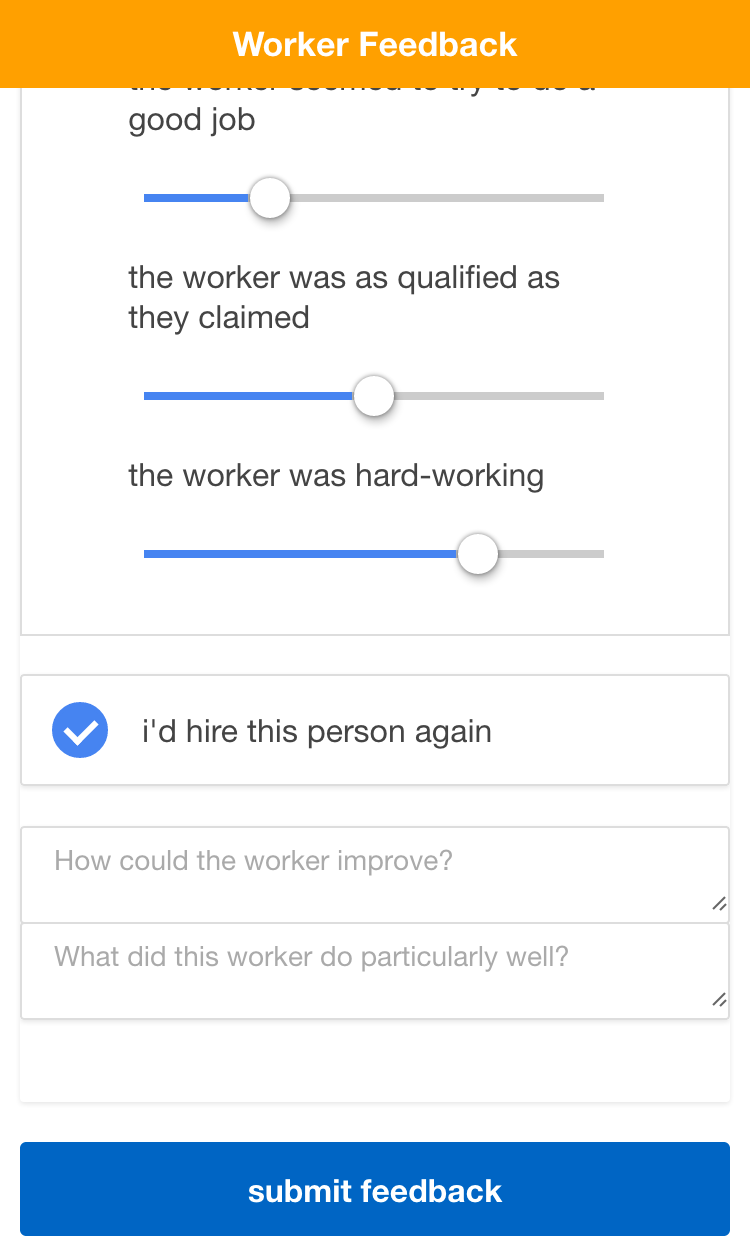
\includegraphics[width=0.25\linewidth]{figures/feedback}
  \end{figure}

\end{frame}

\section[Moving forward]{Where we're going}
\begin{frame}
  \frametitle{Where we're going}
  \begin{itemize}
    \item
    Working on \textbf{collective governance}
    \begin{itemize}
      \item Working with a small group of workers
    \end{itemize}
    \item
    We need to think ahead and build technical system:
    \begin{itemize}
      \item code: \href{https://github.com/alialkhatib/workerCoop}{github $\rightarrow$ alialkhatib/workerCoop}
    \end{itemize}
    \item Interested in contributing (to either)?\\
    \textbf{Contact me} --- \href{mailto:ali.alkhatib@cs.stanford.edu}{ali.alkhatib@cs.stanford.edu}
  \end{itemize}
\end{frame}


\section[Questions, etc\ldots]{Wrap--up}
\begin{frame}
\frametitle{Questions?}
  \begin{itemize}
  \item
  name: \href{https://ali-alkhatib.com}{Ali Alkhatib}
  \item
  email: \href{mailto:ali.alkhatib@cs.stanford.edu}{ali.alkhatib@cs.stanford.edu}
  \item
  twitter: \href{https://twitter.com/alialkhatib_}{@alialkhatib\_}
  \item
  these slides [pdf]:
  {\footnotesize \url{https://al2.in/media/presentations/PlatformCooperativism.pdf}}
  \item
  slide source [\LaTeX]:
  {\footnotesize \url{https://al2.in/media/presentations/PlatformCooperativism.tex}}
  \end{itemize}
\end{frame}

% \section{Thesis}
% \begin{frame}
% \frametitle{Thesis}
% % \framesubtitle{If you take nothing else from my talk, try to remember (and tell people) this}
%   \begin{center}
%     \large{
%       Emerging
%       \texttt{technical} tools are democratizing the creation of (cooperative) labor markets,
%       but we still need to figure out the
%       \textit{social} mechanisms behind successful
%       \textbf{collective governance}.
%     }
%   \end{center}
% \end{frame}

% \section{Challenges to cooperatives}
% % \subsection[]{The Good}
% \begin{frame}
%   \frametitle{Cooperatives are great}
%   % \framesubtitle{Not a very profound or controversial insight}
%     \begin{itemize}
%       \item Good for workers
%       \begin{itemize}
%         \item Fundamentally motivated to meet the needs of its members\\
%               (rather than maximize profit)
%         \item Democratic, transparent decision--making processes
%         \item Collaborative, rather than adversarial, relationships
%       \end{itemize}
%       \item Good for \textit{customers}
%       \begin{itemize}
%         \item Fairer market prices
%         \item Stronger relationships between communities and businesses
%       \end{itemize}
%     \end{itemize}
% \end{frame}

% % \subsection[]{The Bad}
% \begin{frame}
%   \frametitle{\ldots Why are they not more prevalent?}
% We have existence proof that these systems can work
% --- some of them created and operated by people here.

% I argue we haven't figured out how to make success ``formulaic''.
% \end{frame}

% \section{Theory}
% \begin{frame}
% \frametitle{(A confluence of) theoretical underpinnings}
%   \begin{itemize}
%     \item Anthropology, Sociology, and the Social Sciences
%     \begin{itemize}
%       \item Russell Hardin (1982) and \textit{Collective Action}
%       \begin{itemize}
%         \item ``one--shot'' versus ``\textbf{ongoing}'' Collective Action
%       \end{itemize}
%       \item Olson on \textit{The Logic of Collective Action} (1965)
%       \item \textit{Freedom is an Endless Meeting} by Polletta (2012)
%     % \item
%     \end{itemize}
%     \item HCI, CSCW, and CS
%     \begin{itemize}
%       \item Salehi et al. on ``Dynamo'' (2015)
%       \item Stanford Crowd Research Collective on ``Daemo'' (2015)
%       \item Cheng \& Bernstein on ``Catalyst'' (2014)
%     \end{itemize}
%     % \item Design
%     % \begin{itemize}
%     %   \item 
%     %   \item 
%     % \end{itemize}
%   \end{itemize}
    
% \end{frame}

% \section{Methods}
% \begin{frame}
% \frametitle{Methods}
%   % \begin{itemize}
%     % \item Participants
%     % \item Methods
%     \begin{itemize}
%       \item Participant--observation
%       \item Participatory design
%       \begin{itemize}
%         \item B{\o}dker \& Gr{\o}nb{\ae}k (1991)
%         \item Madsen and Aiken (1993)
%       \end{itemize}
%     \end{itemize}
%     % \item Why we can't just ``hack'' this work
%   % \end{itemize}
% \end{frame}

% \section{Mechanisms for collective governance}
% \begin{frame}
%   \frametitle{Useful mechanisms to advance collective governance online}
%   % \framesubtitle{Disclaimer: This is ``working'' knowledge;
%   %                it's only true until we find it's not}
%   \begin{itemize}
%     \item Triggering collective action with thresholds (Catalyst)
%     \item Debate with deadlines (Dynamo)
%     \item Prototyping controversial designs (Daemo)
%   \end{itemize}
% \end{frame}

% \section{Ongoing work}
% \begin{frame}
% \frametitle{Current status}
% \framesubtitle{and call for input}
%   \begin{itemize}
%   \item
%   Still in formative stages of ironing out bylaws and policies.
%   \item
%   If you have experience guiding commons--driven organizations,
%   I would like to hear your insights.
%   \end{itemize}
% \end{frame}

% \section{}
% \begin{frame}
% \frametitle{Wrap--up, questions, contact information}
%   \begin{itemize}
%   \item
%   name: \href{https://ali-alkhatib.com}{Ali Alkhatib}
%   \item
%   email: \href{mailto:ali.alkhatib@cs.stanford.edu}{ali.alkhatib@cs.stanford.edu}
%   \item
%   twitter: \href{https://twitter.com/alialkhatib_}{@alialkhatib\_}
%   \item
%   these slides (PDF):
%   {\footnotesize \url{https://al2.in/media/presentations/CollectiveGovernance.pdf}}
%   \item
%   slide source (\LaTeX):
%   {\footnotesize \url{https://al2.in/media/presentations/CollectiveGovernance.tex}}
%   \end{itemize}
% \end{frame}

\end{document} 